% \documentclass[aspectratio=169,notes]{beamer}
\documentclass[aspectratio=169]{beamer}
\usetheme[faculty=phil]{fibeamer}
\usepackage{polyglossia}
\setmainlanguage{english} %% main locale instead of `english`, you
%% can typeset the presentation in either Czech or Slovak,
%% respectively.
\setotherlanguages{russian} %% The additional keys allow
%%
%%   \begin{otherlanguage}{czech}   ... \end{otherlanguage}
%%   \begin{otherlanguage}{slovak}  ... \end{otherlanguage}
%%
%% These macros specify information about the presentation
\title[MaM]{Mechanics and Machines, Lecture 5} %% that will be typeset on the
\subtitle{Motor sizing (selection)
\\ \        \\ \   
         } %% title page.
\author{Oleg Bulichev}
%% These additional packages are used within the document:
\usepackage{ragged2e}  % `\justifying` text
\usepackage{booktabs}  % Tables
\usepackage{tabularx}
\usepackage{tikz}      % Diagrams
\usetikzlibrary{calc, shapes, backgrounds}
\usetikzlibrary{decorations.pathreplacing,calligraphy,calc,graphs}
\usepackage{amsmath, amssymb}
\usepackage{url}       % `\url`s
\usepackage{listings}  % Code listings
% \usepackage{subfigure}
\usepackage{floatrow}
\usepackage{subcaption}
\usepackage{mathtools}
\usepackage{todonotes}
\usepackage{fontspec}
\usepackage{multicol}
\usepackage{pdfpages}
\usepackage{wrapfig}
\usepackage{animate}
\usepackage{booktabs}
\usepackage{multirow}
% \usepackage{graphicx}
\usepackage{colortbl}

\graphicspath{{resources/}}
\frenchspacing

\setbeamertemplate{caption}[numbered]
\usetikzlibrary{graphs}

% \usepackage[backend=biber,style=ieee,autocite=footnote]{biblatex}
% \addbibresource{biblio.bib}
% \DefineBibliographyStrings{english}{%
%   bibliography = {References},}

\newcommand{\oleg}[2][] {\todo[color=red, #1] {OLEG:\\ #2}}
\newcommand{\fbckg}[1]{\usebackgroundtemplate{\includegraphics[width=\paperwidth]{#1}}}%frame background

\usepackage[framemethod=TikZ]{mdframed}
\newcommand{\dbox}[1]{
\begin{mdframed}[roundcorner=3pt, backgroundcolor=yellow, linewidth=0]
\vspace{1mm}
{#1}
\vspace{1mm}
\end{mdframed}
}

\begin{document}
\setlength{\abovedisplayskip}{0pt}
\setlength{\belowdisplayskip}{0pt}
\setlength{\abovedisplayshortskip}{0pt}
\setlength{\belowdisplayshortskip}{0pt}

\fbckg{fibeamer/figs/title_page.png}
\frame[c]{\setcounter{framenumber}{0}
    \usebeamerfont{title}%
    \usebeamercolor[fg]{title}%
    \begin{minipage}[b][6.5\baselineskip][b]{\textwidth}%
        \textcolor{black}{\raggedright\inserttitle}
    \end{minipage}
    % \vskip-1.5\baselineskip

    \usebeamerfont{subtitle}%
    \usebeamercolor[fg]{framesubtitle}%
    \begin{minipage}[b][3\baselineskip][b]{\textwidth}
        \raggedright%
        \insertsubtitle%
    \end{minipage}
    \vskip.25\baselineskip
}
%   \frame[c]{\maketitle}

\fbckg{fibeamer/figs/common.png}

\note{\scriptsize \begin{itemize}
        \item \ 
    \end{itemize}}

\begin{frame}[t]{Four Key Sizing Factors}
\framesubtitle{}
    \begin{enumerate}
        \item Inertia Ratio: Load Inertia / Motor Inertia (A measurement of how difficult to change the rotating velocity of an object). Nice ratio: (5-10):1
        \item Speed
        \item Max Torque for particular Speed
        \item RMS Torque for particular Speed
    \end{enumerate}
\end{frame}

\begin{frame}[t]{Profiles}
\framesubtitle{}
    \begin{figure}[H]
        \begin{subfigure}{0.59\textwidth}
            \centering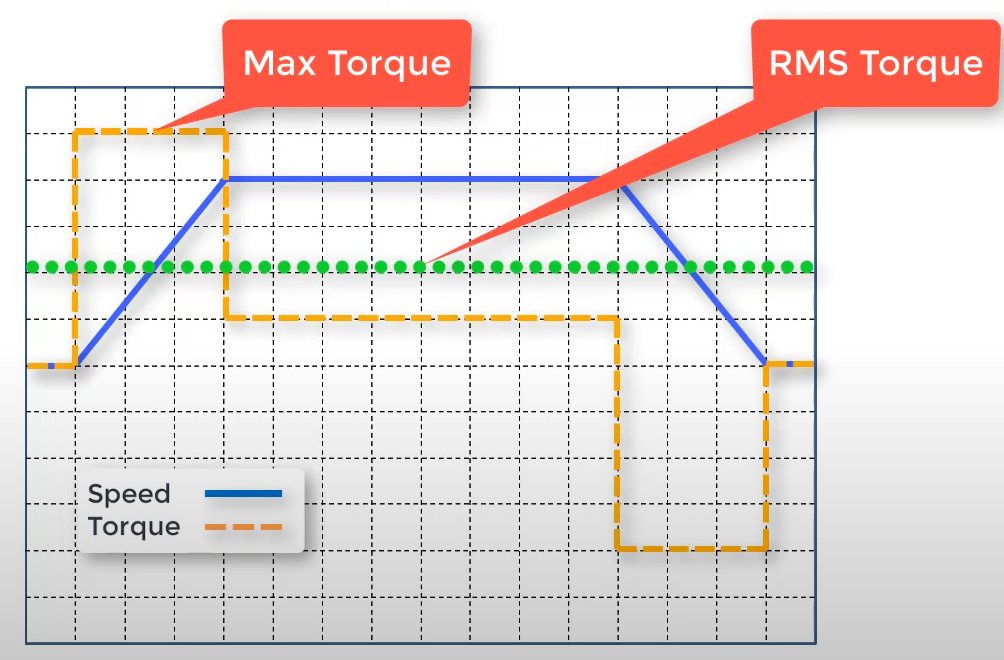
\includegraphics[height=6cm,width=1\textwidth,keepaspectratio]{motor_profile.png}
            % \caption{}
            \label{fig:motor_profile.png}
        \end{subfigure}
        \begin{subfigure}{0.39\textwidth}
            \centering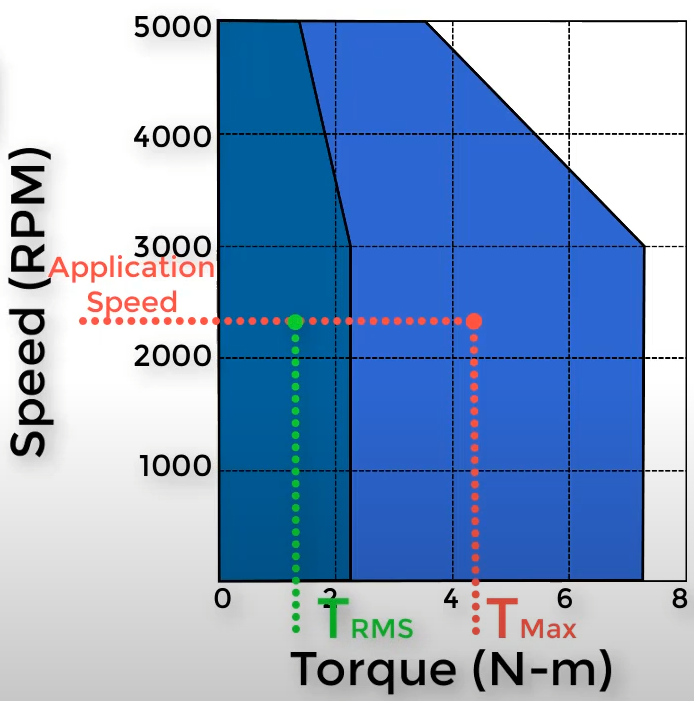
\includegraphics[height=6cm,width=1\textwidth,keepaspectratio]{vel_profile.png}
            % \caption{capture2}
            \label{fig:vel_profile.png}
        \end{subfigure}
    \end{figure}
\end{frame}

\begin{frame}[t]{Motor Selection guideline (Using Simulation)}
    \vspace{-0.5cm }
    \begin{enumerate}
        \small
        \item Determine, what do you want to receive in the end (for instance, a particular R.O. linear velocity and etc).
        \item Create a CAD and Motion Analysis model. Find a load inertia related to a motor axis of rotation.
        \item Define your motion (for example, using table function).
        \item Solve the simulation.
        \item Create plots: $\tau (t)$, $\omega (t)$, others if needed to check the correctness of simulation.
        \item Calculate the power of motor in several position and take the average $P = \omega \tau$ and multiply on some coefficient for reduce sim. error.
        \item Based on the power and size, you can choose the motor.
        \item Start to choose a gearbox (it linearly changes your profile).
        \item If you can, calculate the motor (rotor + gearbox) inertia and find inertia ratio.
    \end{enumerate}
\end{frame}

\begin{frame}[t]{Friction in simulation}
\framesubtitle{}
    \begin{itemize}
        \item \href{https://www.engineeringtoolbox.com/friction-coefficients-d_778.html}{Friction coefficients}
        \item \href{https://docs.sw.siemens.com/en-US/doc/289054037/PL20201105153211099.motion/id563056}{Documentation about 3D contact in NX}
        \item \href{https://docs.sw.siemens.com/en-US/doc/289054037/PL20201105153211099.motion/id562936}{Guidelines for contact materials}
    \end{itemize}
\end{frame}

\begin{frame}[t]{Motors}
\framesubtitle{}
    \begin{itemize}
        \item \href{https://islproducts.com/design-note/how-to-read-dc-motor-gear-motor-performance-curves/}{How to read DC motor Perfomance curves}
        \item \href{https://www.pololu.com/product/3204}{Pololu motors (which are provided)}
        \item \href{https://www.maxongroup.net.au/maxon/view/msp}{Application for motor sizing from Maxon}
        \item \href{https://emanual.robotis.com/docs/en/dxl/mx/mx-28/}{Dynamixel MX-28}
    \end{itemize}
\end{frame}

\begin{frame}[t]{Motor Selection case study}
    \framesubtitle{Video}
    \vspace{-0.6cm}
    \begin{figure}[H]
        \href{https://disk.yandex.ru/d/K9CviPgYnftwrw}{
            \centering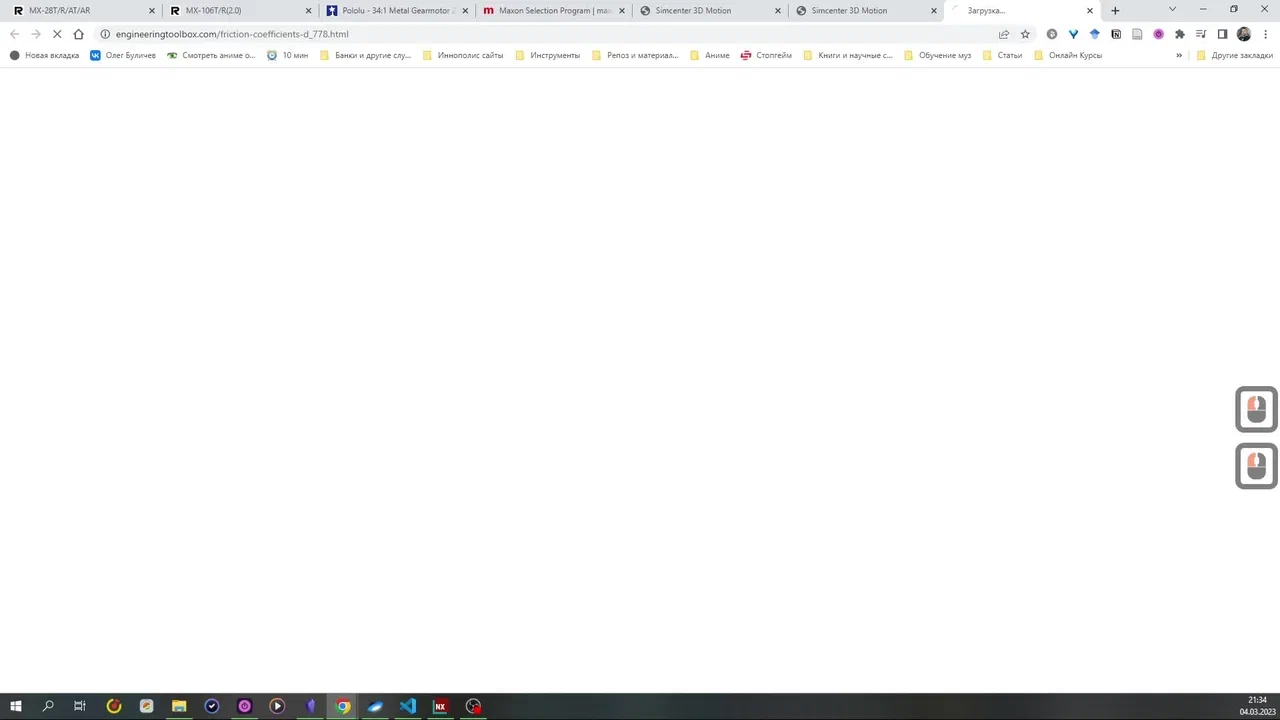
\includegraphics[height=6cm,width=1\textwidth,keepaspectratio]{motor_sizing_preview.png}}
        % \caption{Click on a picture for a video}
        \label{fig:motor_sizing_preview.png}
    \end{figure}
\end{frame}

\begin{frame}[t]{Reference material}
    \framesubtitle{}
    \begin{enumerate}
        \item \href{https://youtu.be/4MaGqSQfYOk}{Servo Motor Sizing Basics Part 1 - Core Concepts (video)}
        \item \href{https://youtu.be/VJFDU31LQGM}{Servo Motor Sizing for Robotic Applications (video)}
    \end{enumerate}
\end{frame}



\fbckg{fibeamer/figs/last_page.png}
\frame[plain]{}

\end{document}